\documentclass[pdf,9pt]{beamer}
\usepackage{listings,graphicx,verbatimbox,hyperref}
\usepackage{hyperref}
\usepackage{bibentry}
\usepackage[customcolors,shade]{hf-tikz}
\newcommand{\N}{\mathbb{N}}
\newcommand{\Z}{\mathbb{Z}}
\newcommand{\Q}{\mathbb{Q}}
\newcommand{\R}{\mathbb{R}}
\newcommand{\C}{\mathbb{C}}

\newcommand{\norm}[1]{\left\lVert#1\right\rVert}
\newcommand{\ceil}[1]{\lceil#1\rceil}
\newcommand{\ov}{\overline}
\newcommand{\cleq}{\preccurlyeq}
\newcommand{\cgeq}{\succcurlyeq}
\newcommand{\bdy}{\textbf{\text{Bdy}}}
\newcommand{\trace}{\text{trace}}
\newcommand{\dom}{\textbf{dom}}
\newcommand{\expec}{\mathbb{E}}
\newcommand{\bigO}{\mathcal{O}}
\newcommand{\tr}{\text{tr}}
\newcommand{\<}{\langle}
\renewcommand{\>}{\rangle}
\newcommand*\oldmacro{}%
\let\oldmacro\insertshorttitle%
% \renewcommand*\insertshorttitle{%
%   \oldmacro\hfill%
%   \insertframenumber\,/\,\inserttotalframenumber}
\DeclareMathOperator*{\argmax}{arg\,max}
\DeclareMathOperator*{\argmin}{arg\,min}

% use the below command to restart numbering in an enumeration, using alphabetics
% \setbeamertemplate{enumerate item}{(\alph{enumi})}
% \setbeamertemplate{enumerate subitem}{(\roman{enumii})}
%\setbeamertemplate{navigation symbols}{}

\usetheme{Warsaw}
\setbeamertemplate{footline}
{
  \leavevmode%
  \hbox{%
  \begin{beamercolorbox}[wd=.3\paperwidth,ht=2.25ex,dp=1ex,center]{author in head/foot}%
    \usebeamerfont{author in head/foot}\insertshortauthor
  \end{beamercolorbox}%
  \begin{beamercolorbox}[wd=.7\paperwidth,ht=2.25ex,dp=1ex,center]{title in head/foot}%
    \usebeamerfont{title in head/foot}\insertshorttitle\hspace*{3em}
    \insertframenumber{} / \inserttotalframenumber\hspace*{1ex}
  \end{beamercolorbox}}%
  \vskip0pt%
}
% \setbeamertemplate{footline}[frame number]
\usepackage{biblatex}
\addbibresource{tetrad.bib}
\bibliography{tetrad}
\usepackage{caption}
\title{Using Machine Learning to Build (Better) Reduced-Order Models of Turbulence}
\author[cmhyett@math.arizona.edu]{Criston Hyett \inst{1}\inst{2} \and Michael Chertkov \inst{1} \and Yifeng Tian \inst{2} \and Daniel Livescu \inst{2} \and Misha Stepanov \inst{1} \and Michael Woodward \inst{1}\inst{2} \and Chris Fryer \inst{2}}
\institute[shortinst]{\inst{1} Program in Applied Mathematics, University of Arizona \and
  \inst{2} CCS-2, Los Alamos National Labs}

\begin{document}
\graphicspath{{./Imgs/}}
%%%%%%%%%%%%%%%%%%%%%%%%%%%%%%%%%%%%%%%%%%%%%%%%%%%%%%%%%%%%%%%%%%%%%%%%%%%%% 

\begin{frame}
  \titlepage
\end{frame}

%%%%%%%%%%%%%%%%%%%%%%%%%%%%%%%%%%%%%%%%%%%%%%%%%%%%%%%%%%%%%%%%%%%%%%%%%%%%%

%%%%%%%%%%%%%%%%%%%%%%%%%%%%%%%%%%%%%%%%%%%%%
\begin{frame}
  \begin{columns}
    \column{0.33\textwidth}
    \begin{centering}
      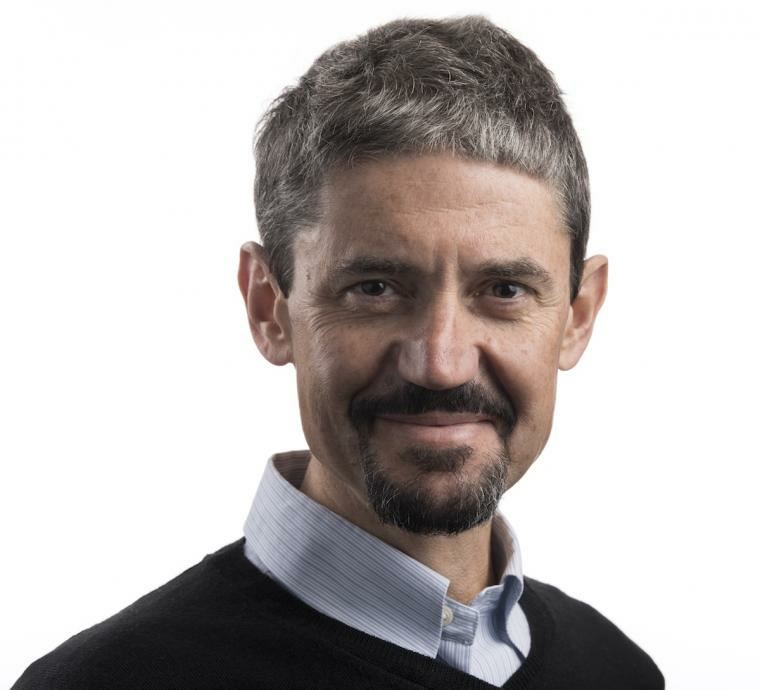
\includegraphics[width=70px]{chertkov.png}
      \\ Misha Chertkov
      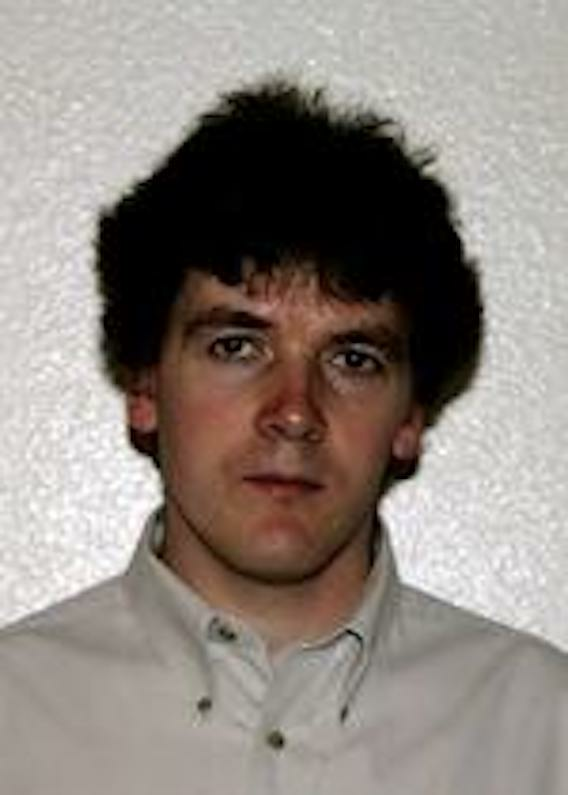
\includegraphics[width=70px]{stepanov.png}
      \\ Misha Stepanov
      \\
    \end{centering}

    \column{0.33\textwidth}
    \begin{centering}
      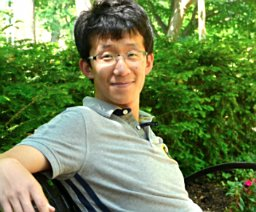
\includegraphics[width=70px]{tian.png}
      \\ Yifeng Tian
      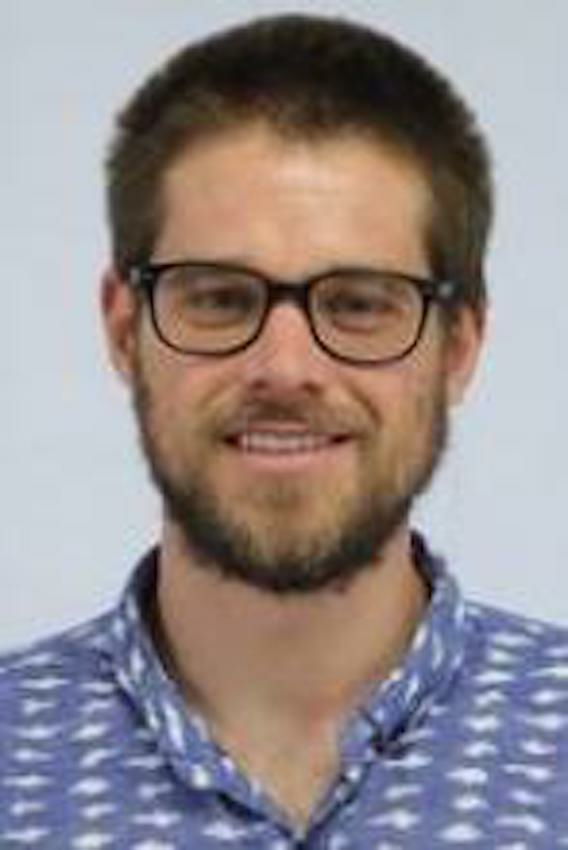
\includegraphics[width=70px]{woodward.png}
      \\ Michael Woodward \\
    \end{centering}

    \column{0.33\textwidth}
    \begin{centering}
      \includegraphics[width=70px]{livescu.png}
      \\ Daniel Livescu
      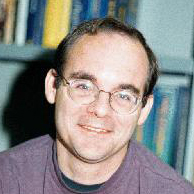
\includegraphics[width=70px]{fryer.png}
      \\ Chris Fryer \\
    \end{centering}

  \end{columns}
\end{frame}
%%%%%%%%%%%%%%%%%%%%%%%%%%%%%%%%%%%%%%%%%%%%%


%%%%%%%%%%%%%%%%%%%%%%%%%%%%%%%%%%%%%%%%%%%%%%%%%%%%%%%%%%%%%%%%%%%%%%%%%%%%% 

\begin{frame}{Why Turbulence?}
  \begin{itemize}
  \item Turbulence is the greatest ``unsolved'' problems in classical physics.
    \begin{itemize}
    \item Work in turbulence dates back to at least Leonardo da Vinci, who visualized voritcies in turbulent flow.
    \item Yet, a full description of the chaotic motion induced from the Navier-Stokes equations - at realistic Reynold's numbers - still eludes even the most powerful supercomputers.
    \end{itemize}

  \item Thus, we look to reduced-order models for computationally tractable approximations to realistic phenomena.

  \end{itemize}
  \vspace{0.25in}
  Our group focuses in particular on using \textbf{physics-informed machine learning} to construct better \textbf{Lagrangian models}. Usually, this manifests as augmenting successful phenomenological models with learnable parameters or functions.
\end{frame}

%%%%%%%%%%%%%%%%%%%%%%%%%%%%%%%%%%%%%%%%%%%%%%%%%%%%%%%%%%%%%%%%%%%%%%%%%%%%% 

%%%%%%%%%%%%%%%%%%%%%%%%%%%%%%%%%%%%%%%%%%%%%%%%%%%%%%%%%%%%%%%%%%%%%%%%%%%%% 

\begin{frame}{Lagrangian Velocity Gradient Tensor}
  \begin{itemize}
  \item The \textbf{Lagrangian velocity gradient tensor (VGT)} is an attractive target of modeling as it is closely related to a variety of important characteristics of turbulence, such as: \textbf{flow topology, deformation of material volume, energy cascade, and intermittency}.
  \item Additionally, we can apply some spatial filtering to create the \textbf{Coarse-Grained Velocity Gradient Tensor}, which provides insight into how these important phenomena on a range of scales.

    \begin{equation}
      A_{ij} = \frac{\partial u_i}{\partial x_j} \to \tilde{A}_{ij} = \frac{\partial \tilde{u}_i}{\partial x_j}
    \end{equation}

  \end{itemize}
\end{frame}

%%%%%%%%%%%%%%%%%%%%%%%%%%%%%%%%%%%%%%%%%%%%%%%%%%%%%%%%%%%%%%%%%%%%%%%%%%%%% 

%%%%%%%%%%%%%%%%%%%%%%%%%%%%%%%%%%%%%%%%%%%%%%%%%%%%%%%%%%%%%%%%%%%%%%%%%%%%% 

\begin{frame}{Governing Equations for VGT}
  We begin with Navier-Stokes for an incompressible fluid:
  \begin{equation} \label{eq:NS}
    \frac{\partial u_i}{\partial t} + u_k \frac{\partial u_i}{\partial x_k} = -\frac{\partial P}{\partial x_i} + \nu \frac{\partial^2 u_i}{\partial x_k \partial x_k}
  \end{equation}
  then, as the velocity gradient tensor is defined as $A_{ij} = \frac{\partial u_i}{\partial x_j}$, we apply spatial derivatives, and use the definition of material derivative ($\frac{dA_{ij}}{dt} = \frac{\partial A_{ij}}{\partial t} + u_k\frac{\partial A_{ij}}{\partial x_k}$) to get:
  \begin{equation}
    \frac{dA_{ij}}{dt} = \frac{\partial A_{ij}}{\partial t} + u_k \frac{\partial A_{ij}}{\partial x_k} = - A_{ik}A_{kj} - \frac{\partial^2 P}{\partial x_i \partial x_j} + \nu \frac{\partial^2 A_{ij}}{\partial x_k \partial x_k}
  \end{equation}
  Additionally, from incompressibility, we have
  \begin{equation}
    \frac{\partial^2 P}{\partial x_k \partial x_k} = - A_{ij}A_{ji}
  \end{equation}
  This allows us to define the nonlocal deviatoric part of the pressure hessian
  \begin{equation}
    H_{ij} = - \left( \frac{\partial^2 P}{\partial x_i \partial x_j} - \frac{1}{3}\frac{\partial P}{\partial x_k \partial x_k}\delta_{ij}  \right)
  \end{equation}
\end{frame}

%%%%%%%%%%%%%%%%%%%%%%%%%%%%%%%%%%%%%%%%%%%%%%%%%%%%%%%%%%%%%%%%%%%%%%%%%%%%% 

%%%%%%%%%%%%%%%%%%%%%%%%%%%%%%%%%%%%%%%%%%%%%%%%%%%%%%%%%%%%%%%%%%%%%%%%%%%%% 

\begin{frame}{Governing Equations for VGT}
  \only<1>{
    We can write the formal (nonlocal) solution for the deviatoric pressure hessian as\footfullcite{ohkitani1995}

  \begin{equation}
    H_{ij}(\textbf{x}) = \iiint \frac{\delta_{ij} - \hat{r_i}\hat{r_j}}{2\pi r^3}Q(\textbf{x} + \textbf{r})d\textbf{r}
  \end{equation}

  Following Lawson \& Dawson\footfullcite{lawson2015}, an expansion of the integral is proposed, first as a Taylor series expansion in $Q(x+r)$
    \begin{equation}
      \hat{H} = \sum_{m,n = 0}^\infty \alpha_{mn}S^mW^n
    \end{equation}
    where
    \begin{equation}
      S = \frac{1}{2}(A + A^T) \qquad W = \frac{1}{2}(A - A^T)
    \end{equation}
  }
  \only<2>{
    Finally we can reduce from an infinite sum using Cayley-Hamilton, and expand via the tensor basis\footfullcite{zheng1993}
    \begin{equation}
      \hat{H} = \sum_{n=1}^{10} g^{(n)}(\lambda_1, \dots, \lambda_5)T^{(n)}
    \end{equation}
    with $g^{(n)}$ scalar functions of the invariants
    \begin{small}
    \begin{equation*}
      \lambda_1 = \tr(S^2) \quad \lambda_2 = \tr(W^2) \quad \lambda_3 = \tr(S^3) \quad \lambda_4 = \tr(W^2S) \quad \lambda_5 = \tr(W^2S^2)
    \end{equation*}
    \end{small}
    and the tensor basis given by:
    \begin{small}
    \begin{align*}
      &T^{(1)} = S &T^{(2)} &= SW-WS\\
      &T^{(3)} = S^2 - \frac{1}{3}I \cdot \tr(S^2) &T^{(4)} &= W^2 - \frac{1}{3}I \cdot \tr(W^2)\\
      &T^{(5)} = WS^2 - S^2W &T^{(6)} &= W^2S + SW^2 - \frac{2}{3}I \cdot \tr(SW^2)\\
      &T^{(7)} = WSW^2-W^2SW &T^{(8)} &= SWS^2 - S^2WS\\
      &T^{(9)} = W^2S^2 + S^2W^2 - \frac{2}{3}I \cdot \tr(S^2W^2) &T^{(10)} &= WS^2W^2 - W^2S^2W
    \end{align*}
    \end{small}
    \textbf{This formulation reduces the challenge to finding the functions of known scalars, i.e., learning the $g^{(n)}$'s}
  }
\end{frame}

%%%%%%%%%%%%%%%%%%%%%%%%%%%%%%%%%%%%%%%%%%%%%%%%%%%%%%%%%%%%%%%%%%%%%%%%%%%%% 

%%%%%%%%%%%%%%%%%%%%%%%%%%%%%%%%%%%%%%%%%%%%%%%%%%%%%%%%%%%%%%%%%%%%%%%%%%%%% 

\begin{frame}{Tensor Basis Neural Network}
  This motivates the use of a neural network to approximate the $g^{(n)}(\lambda_1, \dots, \lambda_5)$, yielding our prediction
  \[
    \hat{H} = \sum_{i=1}^{10}g_{nn}^{(i)}(\lambda_1, \dots, \lambda_5)T^{(i)}
  \]
  We use the usual $L_2$ loss:
  \begin{equation}
    \sum \norm{H - \hat{H}}_2^2
  \end{equation}
  \begin{columns}
    \begin{column}{0.5\textwidth}
      \begin{figure}
        \begin{centering}
          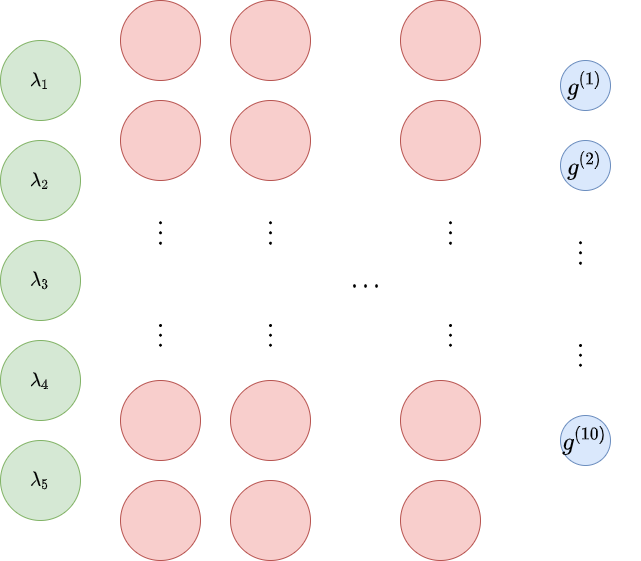
\includegraphics[scale=0.2]{./Imgs/dnn.png}
        \end{centering}
      \end{figure}
    \end{column}

    \begin{column}{0.5\textwidth}
      This tensor basis formulation enforces      
      \begin{itemize}
      \item Galilean Invariant
      \item Rotationally Invariant
      \item Traceless
      \end{itemize}
    \end{column}
  \end{columns}
\end{frame}

%%%%%%%%%%%%%%%%%%%%%%%%%%%%%%%%%%%%%%%%%%%%%%%%%%%%%%%%%%%%%%%%%%%%%%%%%%%%% 


%%%%%%%%%%%%%%%%%%%%%%%%%%%%%%%%%%%%%%%%%%%%%%%%%%%%%%%%%%%%%%%%%%%%%%%%%%%%% 

\begin{frame}{Extension of Previous Work}
  In recent work by Yifeng Tian et.al, they showed capability to predict the evolution of the (Kolmogorov scale) VGT using so-called Tensor Basis Neural Networks (TBNN).

  \begin{figure}
    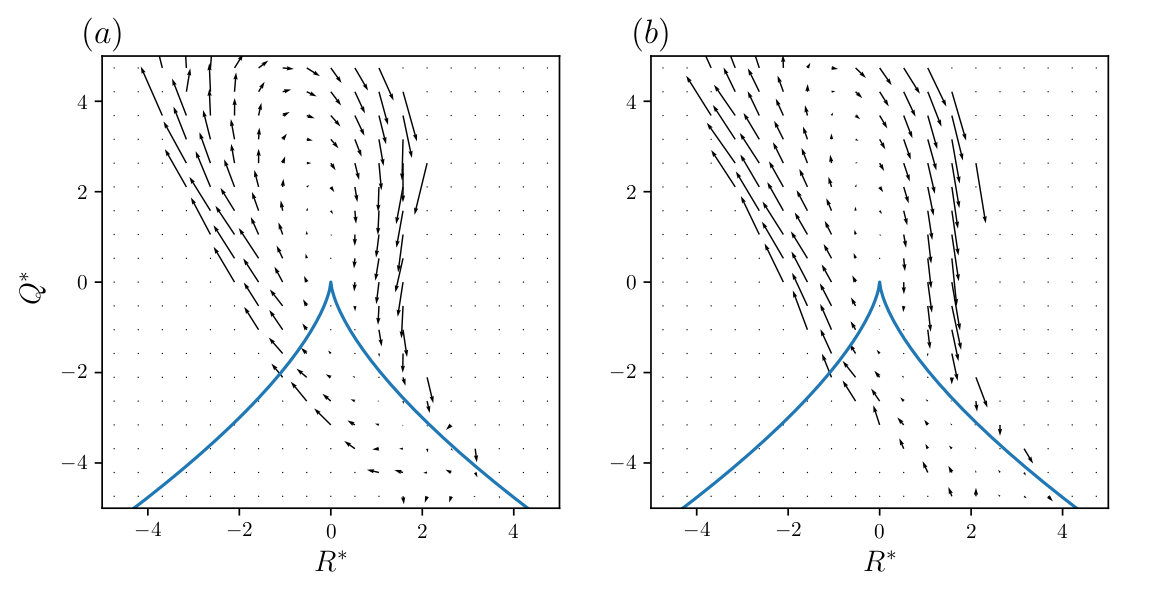
\includegraphics[scale=0.18]{./Imgs/tian_posterioriComparisonVGT.png}
    \caption{Comparison of dynamics in $Q\text{-}R$ phase plane for (a) DNS and (b) Tian et. al's TBNN\footfullcite{tian2021}}
  \end{figure}

\end{frame}

%%%%%%%%%%%%%%%%%%%%%%%%%%%%%%%%%%%%%%%%%%%%%%%%%%%%%%%%%%%%%%%%%%%%%%%%%%%%%

%%%%%%%%%%%%%%%%%%%%%%%%%%%%%%%%%%%%%%%%%%%%%%%%%%%%%%%%%%%%%%%%%%%%%%%%%%%%% 
\begin{frame}{Areas for improvement}
  \only<1>{
    \begin{figure}
      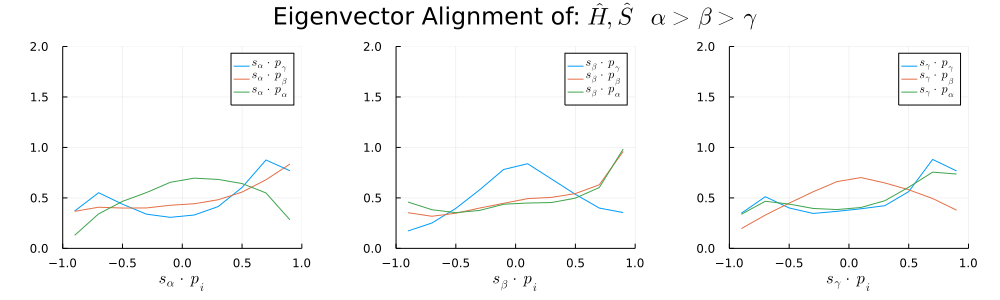
\includegraphics[height=3cm]{pressureStrainAlign_gt.png}
      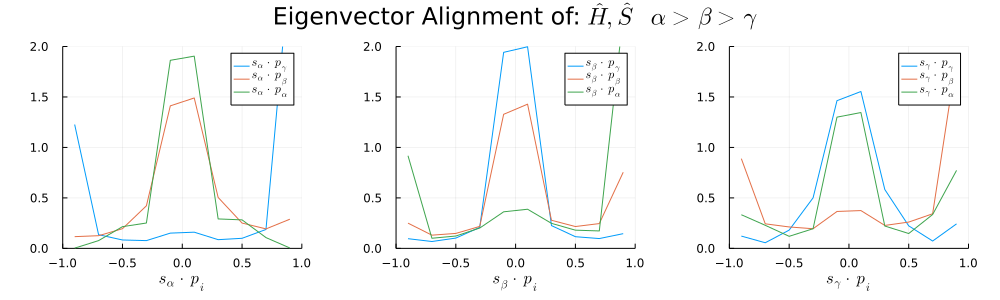
\includegraphics[height=3cm]{pressureStrainAlign_pred.png}
      \caption{The PDF of eigenvector alignment between the pressure Hessian and the strain-rate tensor differs considerably from the ground truth - preferring the extremes of alignment or disalignment. This has implications for the energy cascade.}
    \end{figure}
  }

  \only<2>{
    \begin{figure}
      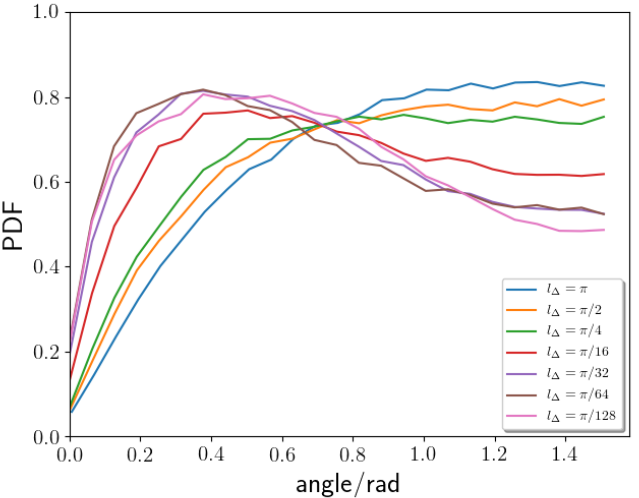
\includegraphics[height=5cm]{tian_CGVGTMisalignment.png}
      \caption{I show here an increasing misalignment between the predicted and ground-truth pressure Hessians for a range of spatial filters\footfullcite{tian2021}. Our eventual goal is to understand this claimed ``performance degradation'' as a function of filtering scale - and remedy it}
    \end{figure}
  }
\end{frame}
%%%%%%%%%%%%%%%%%%%%%%%%%%%%%%%%%%%%%%%%%%%%%%%%%%%%%%%%%%%%%%%%%%%%%%%%%%%%% 


%%%%%%%%%%%%%%%%%%%%%%%%%%%%%%%%%%%%%%%%%%%%%%%%%%%%%%%%%%%%%%%%%%%%%%%%%%%%% 

\begin{frame}{Future Work}
  \begin{itemize}
  \item Our hypothesis currently under testing is that via adding in temporal correlations, e.g. ``memory'', we can refine the predictions of the TBNN to better align across our metrics.
  \item Further, intuitively, larger spatial filters should have longer memory, so we propose to have an adaptive memory kernel, trained per filter size.
  \item Probing the learned functional form of this memory kernel will provide insights into how temporal correlations effect the evolution of the velocity gradient tensor over a range of scales.
  \item Via these extensions, we hope to improve upon the state-of-the-art models of the VGT, while potentially providing new physical insights.
  \end{itemize}
\end{frame}

%%%%%%%%%%%%%%%%%%%%%%%%%%%%%%%%%%%%%%%%%%%%%%%%%%%%%%%%%%%%%%%%%%%%%%%%%%%%% 

\end{document}